% ============================================================================
%  04_experiments.tex --- Sec. 4, the single Experiments section.
%
%  2026-08-30 MERGE PASS.  The former Sec. 4 "Experimental Design" and Sec. 5
%  "Results" are ONE section now: a setting-and-protocol block (shared setting,
%  the two tracks, metrics, reporting) runs straight into the three result
%  subsections, whose titles are unchanged.  Do not re-split them.  The labels
%  sec:setup / sec:protocol / sec:metrics / sec:experiments all now point at
%  this one section.  VERIFIED 2026-08-30: only sec:setup is actually cited
%  (A1_proofs.tex:704, 863); the other three are kept as spare anchors so an
%  appendix cross-reference written against any of the four still resolves.
%
%  Floats: Figure 2 (fig:grid, matched grid, Sec. 4.1), Figure 3 (fig:ordering,
%  ordering + retrieval + fixed-RMSD, Sec. 4.2), Figure 4 (fig:calibration).
%
%  2026-08-30 REFRAME + STATISTICAL REPORTING POLICY.
%    * ZERO t values, ZERO p values, ZERO "significant"/"n.s." in this file.
%      Descriptive standard only: arm mean +/- SEM over independently trained
%      seeds, absolute effect size Delta r, seed counts, and
%      launched/completed/diverged wherever completion differs by arm.
%      Applied in BOTH directions: the favourable statistics went too.
%    * There is NO resolution / step-count sensitivity analysis anywhere in
%      the paper: it was deleted from main text AND appendix.  Do not
%      re-introduce a step count into the narrative; the estimator is named
%      as an ODE integration of the clamped positional flow with Hutchinson
%      divergence estimation, and its settings live in the app:constants row.
%    * The adverse seed imputations are NOT printed here; app:eval carries
%      them and is the actual location of those numbers.
%
%  DESIGN IS ORGANISED BY EVIDENCE TRACK, NOT BY CHRONOLOGY.
%    Track A  matched mechanism grid, 120 parents, six cells.
%    Track B  the conservative held-out endpoint, 93 parents.
%
%  RELOCATED, NOT DELETED: Table 1 -> app:scalediag; the earlier checkpoint
%  family's provenance and the defective scrambled shard -> app:cells,
%  app:data; the adverse seed imputations -> app:eval; the launch timelines
%  and the later cell-D block -> app:p0cells, app:stability;
%  the generation-quality table -> app:generation;
%  the normal-mode family -> app:perturb.
%
%  Every number below is from the verified list.  Matched-grid means never
%  absorb the later relaunch seeds.
% ============================================================================

\section{Experiments}
\label{sec:setup}
\label{sec:protocol}
\label{sec:metrics}
\label{sec:experiments}

Evidence comes from two tracks. \textbf{Track A}, a matched mechanism grid, asks what inside the
value term carries the gain; \textbf{Track B}, a conservative held-out endpoint, asks whether that
gain survives a corrected evaluation and extends to retrieval. Track A is the cleaner design for
causal comparison, its cells differing only in the physics block and the seed; the family behind
Track B has known configuration provenance (\Cref{app:cells}) and is not presented as a matched
trial.

\paragraph{Shared setting.} Every arm trains the bond-free FlowMol3 backbone \citep{flowmol3} on
OMol25 \citep{omol25} against the OMol25/eSEN teacher \citep{esen} under the settings of
\Cref{sec:method}, for $30\,000$ optimiser steps at effective batch $16$, approximately $0.12$ data
epochs. The read-out protocol is fixed and operational: $\log q_\theta$ comes from an ODE integration
of the clamped positional flow with Hutchinson divergence estimation
\citep{ffjord,hutchinson}, and every evaluation energy is a GFN2-xTB single point \citep{gfn2xtb}
from an evaluator that enters no training loss and shares no parameters or functional form with the
teacher. Each held-out parent contributes one group of $K = 9$ geometries, its data geometry plus
$8$ isotropic displacements at $\sigma = 0.15$~\AA{} per coordinate: a local stress test rather than
a thermal conformer ensemble, measuring no mode occupancy.

\paragraph{Track A: the matched mechanism grid.} Six cells at five seeds each, warm-started from a
common checkpoint and matched in \emph{every} non-physics setting: optimiser, budget, batch,
estimator, and shards drawn from the training split alone. The cells are \textbf{A},
flow matching only; \textbf{B}, the same penalty on shards whose energies are \emph{identically
zero}, so \eqref{eq:lvalue} degenerates to $\Var_k[\log q_\theta]$ and no energy label enters the
loss; \textbf{C}, energies scrambled within each parent, a $y$-randomisation
\citep{ruecker2007yrandom} carrying the treatment's own energy multiset and spread; \textbf{D}, true
energies; \textbf{E}, the gradient baseline of \Cref{sec:forcebaseline} alone; \textbf{F}, both, all
scored on 120 held-out parents with the data geometry dropped.

\paragraph{Track B: the conservative held-out endpoint.} Two features of the earlier evaluation
population inflate the contrast, and this endpoint removes both: the data geometry is systematically
its group's lowest-energy member and hence high-leverage, and one perturbation shard read by every
value-supervised arm in that family was built from the split the evaluation parents come from while
the control reads none (\Cref{app:data}). Every geometry was therefore re-scored from one source,
and each per-group
statistic is computed on the \textbf{8 displaced geometries alone} over the \textbf{93 parents
outside the shard pool}; both corrections apply uniformly and both \emph{reduce} the contrast. Five
flow-matching seeds and four completed value seeds enter.

\paragraph{Metrics.} Every statistic is computed inside a parent group and aggregated afterwards,
for the reason the objective is grouped: the per-molecule constant $-\log Z(c)$ would otherwise
dominate a pooled statistic (\Cref{app:eval}). For parent $m$,
\begin{equation}
  r_m = \mathrm{corr}_k\!\left(\log q_\theta(\vx_{m,k}),\, -\tfrac{E_{m,k}}{kT}\right),
  \qquad
  \mathrm{NRV}_m = \frac{\Var_k[\log q_\theta(\vx_{m,k}) + E_{m,k}/kT]}
       {\Var_k[E_{m,k}/kT]} .
  \label{eq:rm}
\end{equation}\vspace{-6pt}%
Pearson $r_m$ is invariant under positive affine maps of either variable (\Cref{rem:affine}), so it
scores the \emph{shape} of $\log q_\theta$ against energy and is blind to calibration.
$\mathrm{NRV}_m$ is invariant to the per-group constant \Cref{prop:ident} leaves free and is
anchored at both ends: a within-group Boltzmann density scores $0$, a \emph{constant} log-density
exactly $1$. The identity $\mathrm{NRV}_{\min} = 1 - r_m^2$ is the best any single rescaling could
reach, and $kT_{\mathrm{eff}}$ is the implied temperature, ideally $1.0$~eV (\Cref{app:scalediag}).
\emph{Retrieval} asks how often ranking a parent's geometries by $\log q_\theta$ puts the
lowest-energy one first, or in the top three.

\paragraph{Reporting.} We report effect sizes, means and standard errors over independently trained
seeds, together with every seed-level result. Because several cells contain only two to five
completed seeds and completion is objective-dependent, we use these descriptive quantities rather
than treating asymptotic null-hypothesis tests as the primary evidence. A training run is the unit
of replication, every figure draws every seed point, every value-cell mean carries its launched /
completed / diverged counts, and per-seed records are in \Cref{app:p0cells,app:eval,app:stability}.

Two quantities run through the results below: a correlation, which scores the \emph{direction} of the
density's response to energy, and a normalised residual variance, which also scores its
\emph{magnitude}. Value supervision moves the first and not the second. Relative basin mass, the
third property of \Cref{sec:theory}, is measured nowhere.

\subsection{Correct Energy Pairings Drive the Gain}
\label{sec:ablation}
\label{sec:negative}

\Cref{fig:grid} answers three questions with one matched design. \emph{Does the value term improve
ordering?} Cell D reaches $0.421 \pm 0.016$ against cell A's $0.217 \pm 0.008$, $\Delta r = +0.204$,
and every completed D seed lies above the observed range of every control cell. \emph{Is the gain
merely density regularisation?} Cell B, whose shard energies are identically zero so no energy label
enters the loss, reaches $0.187 \pm 0.030$, $0.030$ \emph{below} A, and D exceeds it by $+0.234$.
\emph{Does it require the correct correspondence?} Cell C, carrying real energies whose pairing to
geometries is destroyed, sits at $0.185 \pm 0.020$, again below no physics, and D exceeds it by
$+0.236$. The three controls lie within $0.032$ of one another, an order of magnitude below the
treatment effect: the geometry-to-energy correspondence moves ordering, an auxiliary penalty on the
log-density or the energy multiset alone does not.

% figures/fig3_grid.tex -- float wrapper for FIGURE 3, the matched six-cell grid.
%
% Image produced by figures/fig3_grid.py (PDF at figures/out/fig3_grid.pdf,
% audit record at figures/out/fig3_grid_data.json).  Drawn at final size
% (5.5in single column); include with width=\linewidth only, never \resizebox.
%
% PROVENANCE.  Every number in the image is recomputed at build time from
% runs/eval_ours/clean_p0_<CELL>_s<N>/boltz_independent_records.csv by the
% recipe "drop pert_id == 0, keep xtb_ok, per-parent Pearson r(log q_theta, -E/kT),
% mean over the 120 parents"; the launched/completed/diverged triples are a
% checkpoint census over runs/p0/p0_<CELL>_s<N>.  The generator refuses to draw
% unless all 24 per-seed values, all six cell means/sems, all six triples and
% all six contrasts reproduce the independently verified values.  The Welch t
% values stay inside that gate and inside the audit JSON; none is rendered.
%
% RULINGS SATISFIED.  (i) This float replaces the per-seed grid table in the
% main text: the numeric table is not the communication device, the seed points
% are.  (ii) The verified force cell is clean_p0_E_force_*, not E2; the post-hoc
% relaunches D_energy_s6/s7/s9 and F_both_s6..s10 are excluded, because no
% diverged seed is ever replaced.  (iii) The reference-included
% mean_pearson_r in boltz_independent.json is never read.  (iv) NO inferential
% statistic is rendered anywhere in this float.  Panel (b) is an EFFECT-SIZE
% panel: six differences of cell means with the propagated standard error of
% the difference as a descriptive whisker.  No Welch t, no p-value, and no
% "significant" / "n.s." label appears in the image or in the caption.
%
% C11 (this pass).  Panel (a)'s title now conditions on completion explicitly
% ("Among completed runs, ..."), and the caption no longer offers survivorship
% as an alternative reading of cell D.  The claim it makes instead is checkable:
% the three completed D seeds (0.452, 0.398, 0.412) lie above every control
% seed (A max 0.234, B max 0.243, C max 0.232), and the direction agrees with
% the corrected earlier checkpoint family, whose 93-parent primary endpoint is
% 0.369 (value) vs 0.200 (FM only) in figures/out/scale_primary.json
% -> dropref/{a3_energy,a1_fm_only}/per_seed/*/primary_93/pearson_r.  What the
% caption does NOT claim is an unconditional magnitude for D or F.
% C12 (figure-editor pass, reviewer item 8).  The PDF is placed at
% width=\linewidth again, as this header always specified, and the generator
% draws its canvas at exactly 5.50 x 2.35 in with an explicit (non-tight)
% bounding box.  Placed size therefore equals drawn size, every in-figure point
% size is a page point size, and nothing renders below 7 pt.  The canvas height
% is the height the float already occupied (3.05 in x 0.76 = 2.318 in), so the
% vertical footprint is unchanged; the enlargement comes entirely from the 24%
% of the column that the fractional placement used to waste as margin.  The
% in-panel line repeating "120 held-out parents / reference geometry dropped /
% independent GFN2-xTB evaluator" is deleted: the caption below states all three
% and the line was the least legible object on the page.
\begin{figure}[t]
\begin{center}
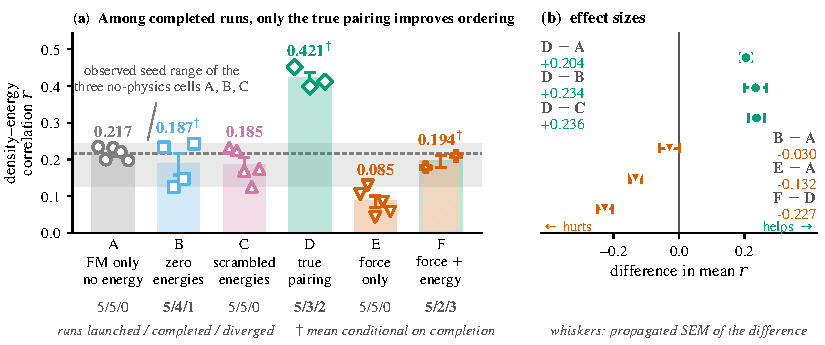
\includegraphics[width=\linewidth]{figures/out/fig3_grid.pdf}
\end{center}
\caption{Archived readout results; likelihood labels in the plots refer to $\widehat\ell_\theta$, not a validated generator density. \textbf{A matched six-cell grid isolates what the energy term
contributes.} Population: 120 held-out parents, reference geometry dropped, 8
displaced geometries each, scored by an independent GFN2-xTB evaluator, not the
eSEN training teacher. Metric: the per-parent density--energy correlation $r$,
per cell as the mean over completed training seeds (whisker: standard error
over seeds) with every completed seed drawn, and in (b) as effect sizes:
differences of cell means, whiskers the propagated descriptive SEM of the
difference rather than a confidence interval. Cells A--F are defined in
\Cref{sec:ablation}; runs launched / completed / diverged are printed under each
cell, because completion is objective-dependent. Only the true geometry--energy
pairing separates: every completed D seed lies above the shaded band, the
observed seed range of A, B and C; the zero-energy and scrambled cells do not,
and the gradient baseline falls below. \textbf{Cells B, D and F lost seeds to divergence}
($\dagger$), so their means are conditional on completion and the D and F
unconditional magnitudes are not identified. Panel detail in
\Cref{app:figdetail}.}
\label{fig:grid}
\end{figure}


\textbf{The gradient comparator.} Cell E carries the score-matched force term alone, completed $5/5$
at $0.085 \pm 0.016$, below the physics-free baseline by $-0.132$; added to the value term it
subtracts again, F scoring $0.194 \pm 0.016$ against D's $0.421$, a difference of $-0.227$. Cell E2,
identical to E at $\lambda_1 = 0.01$, completed $5/5$ at $0.080 \pm 0.013$, so the result does not
rest on one badly chosen weight (\Cref{app:p0cells}). The claim stays narrow. Under this implementation's endpoint
parameterisation these cells match a score equal to $(1-t)$ times \eqref{eq:score}
(\Cref{app:forcemech}); what is measured is that comparator --- naive, off-policy, endpoint --- on
this non-equilibrium corpus, and not \eqref{eq:score} at the scale it defines. It is not a claim that force supervision is unhelpful for
energy-grounded generation, which can be made to work \citep{psm,driftingboltzmann}; \Cref{prop:trap,prop:conflict}
name candidate mechanisms. Two forward-only diagnostics on the shared warm-start checkpoint locate
the difficulty: the endpoint force is a poor target at the interpolant, where the force actually
acting is nearly orthogonal to it (per-atom cosine $0.16$ at $t^{*} = 0.85$) because the
interpolant sits off the data manifold, and the force term's parameter gradient points
systematically against the flow-matching gradient while the value term's is close to orthogonal to
it. We read these as a measured mechanism for the observed difference rather than a proof
(\Cref{app:forcemech}).

\textbf{Completion by cell.} The launch record is A $5/5/0$, B $5/4/1$, C $5/5/0$, D $5/3/2$, E
$5/5/0$, F $5/2/3$ launched / completed / diverged: none of the ten runs without the value term
failed, against six of the twenty carrying it, cell B included, which implicates the reverse-time
log-density objective and its gradient rather than the teacher's energies; D and F are means over
survivors. Two records bound that risk. A later, byte-identically configured block of four cell-D
seeds completed in full at $0.353$, $0.374$, $0.452$ and $0.471$, and across all seven scored D runs
the mean is $0.416 \pm 0.017$; that block is reported separately and never merged into the grid
means. The F campaign launched $10$, completed $3$ and diverged $7$, its three completed runs
agreeing at $0.197 \pm 0.009$ (\Cref{app:p0cells,app:stability}).

\subsection{The Gain Generalises to Held-out Molecules and Retrieval}
\label{sec:mainresult}
\label{sec:main}
\label{sec:reference}

\textbf{Ordering improves well beyond seed spread.} On the conservative held-out endpoint ---
$93$ parents disjoint from the supervision pool, data geometry dropped, every geometry scored by the
independent evaluator --- the value term raises the mean per-parent correlation between
$\log q_\theta$ and $-E/kT$ from $0.200 \pm 0.018$ over five flow-matching seeds to
$0.369 \pm 0.023$ over four completed value seeds, an effect size of $\Delta r = +0.169$
(\Cref{fig:ordering}a). All four value seeds exceed all five control seeds, so the observed seed
ranges of the two arms do not overlap. The launch record is $5/5/0$ for flow matching and $5/4/1$
for the value arm, so the value mean is conditional on four of five completed launches, and
\Cref{app:imputation} reports conservative imputations for that run. The shift is spread across
the population rather than carried by a few parents, value supervision scoring higher on $67$ of the
$93$ (\Cref{fig:ordering}b).

\textbf{Retrieval improves, and the gain persists at fixed RMSD.} Ranking a parent's eight
displaced geometries by $\log q_\theta$ identifies the lowest-energy one $29.6\%$ of
the time under value supervision against $20.2\%$ for the control, with $12.5\%$ at chance, and
top-3 rises from $49.5\%$ to $62.4\%$ against $37.5\%$ (\Cref{fig:ordering}c). Retrieval is
invariant to the per-group constant and to calibration. The gain also persists at fixed RMSD: on a family
holding the within-group displacement magnitude constant to numerical precision, value supervision
reaches $0.305$ against $0.182$, a gap of $+0.124$ with four seeds per arm (\Cref{fig:ordering}d),
which rules out radial-distance variation as the sole explanation. A normal-mode family also has a
positive mean gap ($+0.185$ over five seeds per arm), but its observed seed ranges overlap, so we
treat it as supporting context only (\Cref{app:perturb}).

% figures/fig2_ordering.tex -- float wrapper for the held-out ordering figure
% (FIGURE 3 in the rendered PDF; cited as \Cref{fig:ordering} from Sec. 5.2).
% Image produced by figures/fig2_ordering.py, which also writes
% figures/out/fig2_ordering_data.json recording every plotted number and the
% file it came from.
%
% NOTATION.  Every drawn label reads \log q_\theta, the clamped positional-flow
% density (endpoint discrete labels held fixed, positional ODE reversed).  It is
% not the joint generator's conditional density and the caption says which
% quantity it is.  The stored record files keep the column name log_p_theta;
% that is a data-file field name and is never drawn.
%
% PROVENANCE
%   panel (a)  figures/out/scale_primary.json, ["dropref"][arm]["per_seed"]
%              [seed]["primary_93"]["pearson_r"], cross-checked at build time
%              against runs/eval_ours/wide_*/boltz_records.csv (both routes
%              agree to 4 decimals; the generator asserts it).
%   panel (b)  runs/eval_ours/wide_*/boltz_records.csv, pert_id 0 dropped,
%              restricted to the 93 ids in figures/out/primary_endpoint.json.
%   panel (c)  figures/out/retrieval_utility.json, ["primary_93"] blocks.  The
%              file's ["oracle"] key is renamed on load: the quantity is the
%              independent evaluator scoring the eSEN TRAINING TEACHER, i.e. an
%              ensemble-specific teacher-evaluator agreement reference, and that is what
%              the legend says.  Its numeral is not printed in the figure.
%   panel (d)  Gaussian side: the same records as (a).  Fixed-RMSD side: the
%              verified pair (value 0.305, flow matching 0.182, gap +0.124,
%              four seeds per arm) carried as constants in the generator.
%              See the ruling below.
%
% RULINGS HONOURED
%   * PANEL (d) IS DRAWN, AND ITS LIMIT IS DRAWN WITH IT.  No artefact under
%     runs/eval_p3 reproduces the verified fixed-RMSD aggregation -- the __cpu
%     round (40 parents, 4 seeds/arm) gives 0.3028 / 0.1885 and the __gpu60
%     round (120 parents, 4 seeds/arm) 0.3505 / 0.2482 -- so the panel plots the
%     verified ARM MEANS ONLY, prints the seed count, draws no per-seed cloud on
%     that side, and says in the panel that the two families are separate rounds
%     on different parent sets and that the comparison is between the gaps.
%     Splicing another round's per-seed cloud under the verified means would be
%     a cross-round comparison and is not done.
%   * The standardised geometry-level scatter that used to be panel (c) is
%     REMOVED.  Its fitted coefficient was algebraically the panel-(a) arm mean,
%     so it restated a number two other panels already carried, and the
%     fixed-RMSD control answers a claim-threatening confound that no other
%     panel addresses.
%   * The scrambled-energy arm is REMOVED from panel (a): only one of its two
%     shards was scrambled, so it is defective, and cell C of \Cref{fig:grid}
%     supersedes it.  No number that the verified register does not carry is
%     drawn anywhere in this figure.
%   * Every arm with three to five seeds shows its raw seed points -- panels
%     (a), (c) and the Gaussian half of (d).
%   * Every "ceiling" and "oracle" label is gone.  The orange marker in panel
%     (c) is the teacher-evaluator agreement reference, labelled ensemble-specific.
%   * NO INFERENTIAL STATISTIC IS DRAWN.  The reporting standard is descriptive:
%     arm means over independently trained seeds, the standard error over those
%     seeds, every raw seed point, the absolute gain Delta r, the seed counts,
%     and the launched/completed/diverged record.  The Welch t and the exact
%     permutation p are still computed as pipeline guards and are written to
%     figures/out/fig2_ordering_data.json, but no t value, no p-value and no
%     significance label reaches the image or the caption.
%   * Palette semantics are the fixed ones: grey = FM-only baseline,
%     green = value/energy.  Vermilion (force) does not appear -- the
%     gradient-supervision baseline is argued in Sec. 5.3.
%   * WIDTH.  This float places the PDF at \linewidth = 5.50 in and the
%     generator DRAWS at 5.50 in (FULL_W = PLACED_FRACTION * TEXTWIDTH_IN with
%     PLACED_FRACTION = 1.00), so the scale on the page is 1.000 and every
%     in-figure point size is a true page point size, none below 7 pt.  An
%     earlier 0.76 placement of a 5.5 in canvas shrank every size to 76% of
%     what the generator asked for; do not go back to it.  Do not \resizebox
%     this float, and if the placement here ever changes, change
%     PLACED_FRACTION in the generator to match.
\begin{figure}[t]
\begin{center}
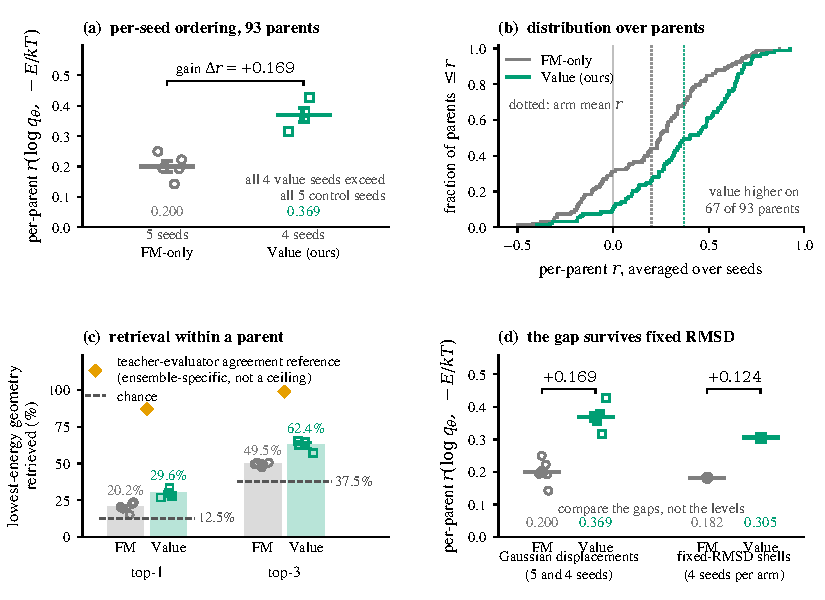
\includegraphics[width=\linewidth]{figures/out/fig2_ordering.pdf}
\end{center}
\caption{Archived readout results; likelihood labels in the plots refer to $\widehat\ell_\theta$, not a validated generator density. \textbf{Energy-value supervision improves local density--energy ordering.}
Population for \textbf{(a)}--\textbf{(c)}: the 93 held-out parents disjoint from the value term's
shard pool, data geometry dropped, up to eight displaced geometries each, scored by GFN2-xTB, an
evaluator independent of the eSEN potential that supplied the training energies. The metric is the
per-parent correlation between the clamped positional-flow density $\log q_\theta$ and $-E/kT$.
\textbf{(a)} Every seed of both arms; rules are arm means, bars their standard error over seeds,
and the gain is $\Delta r = +0.169$ with all four value seeds above all five control seeds. The
value arm is $5/4/1$ launched / completed / diverged, so its mean is conditional on completion.
\textbf{(b)} The shift is spread across the population rather than carried by a few parents.
\textbf{(c)} Ranking a parent's geometries by $\log q_\theta$ retrieves the lowest-energy one more
often; the orange marker is the teacher-evaluator agreement reference (not a ceiling): that
evaluator scoring the training teacher, ensemble-specific and re-measured for any other ensemble.
\textbf{(d)} Holding the within-group displacement magnitude constant to numerical precision leaves
the gap in place, so distance variation is not sufficient to explain the gain; that family is a
separate evaluation round on its own parents with four seeds per arm, and only its arm means are
plotted, so the comparison to make is between the two gaps, not between the two levels. Panel detail in \Cref{app:figdetail}.}
\label{fig:ordering}
\end{figure}


\textbf{Where the level sits.} Teacher and evaluator are different theories of chemistry, so a model
reproducing its teacher exactly would not score $1$: pushing the \emph{teacher's own} energies
through the identical pipeline gives $r = 0.927$ on the same 93 parents, an ensemble-specific
reference, not a ceiling (\Cref{app:scalediag}). Budget and locality remain open explanations of the
rest.

\subsection{Value Supervision Improves Ordering Before Calibration}
\label{sec:scale}

\textbf{Direction improves; the raw scale does not.} Ordering and calibration are different requests
of the same density, and the objective clearly answers the first. On the same models, seeds and
parents, the normalised residual variance rises from $1.402$ to $2.144$, where a \emph{constant}
log-density scores exactly $1$ (\Cref{fig:calibration}a): the arm that ranks geometries better sits
further from the Boltzmann scale, which is why we report the two quantities separately rather than
as one claim of physical grounding.

\textbf{The usable signal nonetheless increases.} No rescaling can bring a parent's
$\mathrm{NRV}_m$ below $1 - r_m^2$, and that optimally rescaled bound falls from $0.825$ to $0.747$
(\Cref{fig:calibration}b), so the density carries more energy-aligned information than before. The implied temperature moves the same way, from
$kT_{\mathrm{eff}} = 8.02$~eV to $2.34$~eV against the $1.0$~eV target (\Cref{fig:calibration}c),
and so does the slope, from $0.130$ to $0.448$: a response that was far too flat moves to the right
order of magnitude, overshooting rather than approaching. The same separation
appears against the eSEN training teacher, where $r$ rises from $0.202$ to $0.399$ while raw NRV
rises from $1.676$ to $2.821$ (\Cref{app:scalediag}).

\textbf{What is left is an optimisation gap, not a missing term.} Raw NRV additionally charges for
the part of the residual that is not energy-aligned, and that part grows enough to push NRV up even
as the rescaled bound falls; the free constant per group is not the cause, since $\mathrm{NRV}$ is
invariant to it. Both parts are already what \eqref{eq:lvalue} asks for. Writing
$\log q_\theta = a\,(-E/kT) + b + \varepsilon$ within a group, with $\varepsilon$ uncorrelated with
$E$ by construction, gives
\begin{equation}
  \Var_k\bigl(\log q_\theta + E/kT\bigr) \;=\; (a-1)^2\,\Var_k\bigl(E/kT\bigr) \;+\; \Var_k(\varepsilon),
  \label{eq:scaledecomp}
\end{equation}
whose two terms are exactly the magnitude of the response and its energy-unaligned component, and
which is minimised uniquely at $a = 1$ with $\Var_k(\varepsilon) = 0$. The variance form annihilates
the free constant $b$ but not the slope $a$: \eqref{eq:lvalue} already demands a calibrated
response, not merely a correctly ordered one. What we report is therefore not a term missing from
the objective but a gap between what it asks for and what this training run reached, and the
slope moving from $0.130$ to $0.448$ is movement along that axis rather than orthogonal to it. How far the slope can be driven by weighting the value term
more heavily, or by spending more of the budget on it, is a question these experiments leave open.\label{sec:generation}\ On generation itself we detect \emph{no
degradation in validity, PoseBusters pass rate \citep{posebusters} or uniqueness} at the evaluated
sample size (\Cref{app:generation}).

% figures/fig4_calibration.tex -- float wrapper for Figure 4 (Sec. 5.4).
% Image produced by figures/fig4_calibration.py, which also writes
% figures/out/fig4_calibration_data.json recording every plotted number and the
% file it came from.
%
% REVISION C6 (correctness fix, applied 2026-08-14)
%   The previous version overlaid the continuous curve NRV = 1 - r^2 on a plane
%   whose points are (mean-over-parents r, median-over-parents NRV).  That curve
%   is not a valid boundary for such an aggregate: the identity is per parent,
%   NRV_min(m) = 1 - r_m^2, and mean_m[1 - r_m^2] != 1 - (mean_m r_m)^2.  The
%   curve has been REMOVED.  The optimally rescaled bound is now reported the
%   only way it can be reported honestly, as its own per-seed aggregate, in the
%   new panel (b).  The generator asserts the per-parent identity at build time.
%   The teacher point is now labelled the TEACHER-EVALUATOR AGREEMENT REFERENCE
%   (the independent evaluator scoring the training teacher), never a ceiling.
%
% PROVENANCE (every number machine-read; nothing transcribed from prose or PDF)
%   all panels  figures/out/scale_primary.json, ["dropref"][arm]["per_seed"]
%               [seed]["primary_93"].  Panel (a) uses "pearson_r" (MEAN over the
%               93 parents) and "nrv" (MEDIAN over parents); panel (b) uses
%               "nrv" and "nrv_min" (MEAN over parents); panel (c) uses
%               "T_eff_eV" (kT divided by the median per-parent slope).
%               All four are cross-checked at build time against the per-parent
%               blocks of runs/eval_ours/calibration/calibration_dropref.json
%               restricted to the 93 ids in figures/out/primary_endpoint.json;
%               the two routes agree to 4 decimals and the generator asserts it.
%   reference   runs/eval_ours/ceiling_full_dropref/ceiling_per_group.csv,
%               restricted to the same 93 ids.  Its r = 0.9271 is the verified
%               number; its NRV = 0.082, NRV_min = 0.095 and kT_eff = 1.25 eV
%               were DERIVED for this figure from that file under the same
%               aggregation conventions as the model arms, and the caption says
%               so.
%
% RULINGS HONOURED
%   * No 1 - r^2 curve (revision C6).
%   * The three properties stay separated: this figure measures local ordering
%     and local calibration only.  Global mass allocation is not measured
%     anywhere in the paper and no panel here implies otherwise.
%   * Every arm shows its raw seed points: 4 open markers per arm in all three
%     panels (five for the flow-matching control), with the filled marker or rule
%     the arm mean over seeds and the
%     bar its standard error over seeds.
%   * The orange point is a reference, not a ceiling.  The figure labels it
%     "teacher-evaluator agreement" and prints its two numbers; what it is and is not is
%     stated in the caption, where it can be read at caption size.
%   * No p-value is printed here; the primary contrast statistics live with
%     Figure 2 and Table 1.
%   * Palette semantics are the fixed ones: grey = FM-only baseline,
%     green = value supervision, orange = teacher-evaluator agreement.
%     Vermilion (force) does not appear; the gradient-supervision baseline is
%     argued in Sec. 5.3.
%   * Drawn at final size (5.5 x 2.10 in) with an explicit, non-tight bounding
%     box; included with width=\linewidth, never rescaled.  Placed size equals
%     drawn size, so every in-figure point size is a page point size and nothing
%     renders below 7 pt.
%
% C12 (figure-editor pass, reviewer item 8).  The float placed this PDF at
% 0.76\linewidth while the canvas was drawn at 5.5 in, so in-figure type
% rendered at 76% of its stated size.  The placement is back to \linewidth and
% the canvas height is the height the float already occupied (2.72 x 0.76 =
% 2.067 in), so the vertical footprint is unchanged and the panels grow into the
% column width the fractional placement was wasting; panel (c) goes from 0.61 to
% 0.98 in wide.  The teacher-evaluator agreement annotation is cut to the two
% numbers, with what the point is and is not moved into the caption.  Every
% temperature label reads kT_eff, which is what the quantity is: an energy in
% eV, kT divided by the fitted slope, against a numerical kT = 1.0 eV target.
\begin{figure}[t]
\begin{center}
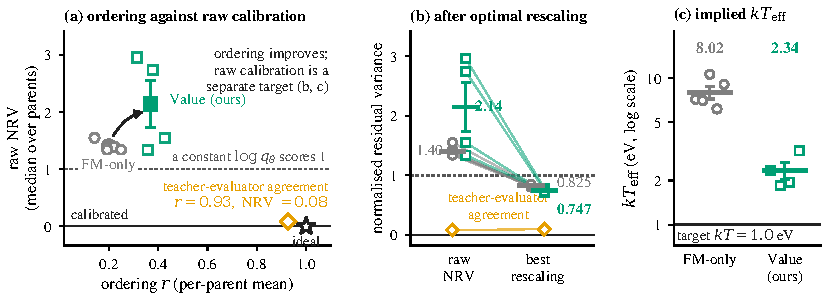
\includegraphics[width=\linewidth]{figures/out/fig4_calibration.pdf}
\end{center}
\caption{Archived readout results; likelihood labels in the plots refer to $\widehat\ell_\theta$, not a validated generator density. \textbf{Value supervision improves ordering before calibration.}
Same 93 held-out parents as \Cref{fig:ordering}, reference geometry dropped, GFN2-xTB evaluator;
five seeds for the flow-matching control, four for the value arm (open markers; filled marker or
rule the arm mean, bar its standard error over seeds). Metrics: ordering $r$ against raw
calibration $\mathrm{NRV} = \mathrm{Var}(\log q_\theta + E/kT)/\mathrm{Var}(E/kT)$ \textbf{(a)},
the optimally rescaled residual $\mathrm{NRV}_{\min}$ \textbf{(b)}, and the implied
$kT_{\mathrm{eff}}$ \textbf{(c)}. Three diagnostics move toward the Boltzmann-consistent regime:
$r$ rises from $0.200$ to $0.369$, $\mathrm{NRV}_{\min}$ falls from $0.825$ to $0.747$, and
$kT_{\mathrm{eff}}$ moves from $8.02$ to $2.34$~eV toward the $kT = 1.0$~eV target. Raw residual
variance --- the diagnostic most directly aligned with the objective as displayed --- remains a
separate unmet target: NRV rises from $1.402$ to $2.144$, past the $1$ that a constant
log-density scores, showing that errors in response magnitude and energy-unaligned variation
remain even as ordering improves. The value arm ($5/4/1$ launched / completed / diverged) is
conditional on completion. The orange marker is the teacher-evaluator agreement reference (not a
ceiling); panel detail and its derivation are in \Cref{app:figdetail}.}
\label{fig:calibration}
\end{figure}

